\documentclass[tikz,border=10pt]{standalone}

\usepackage{amsmath}
\usetikzlibrary{arrows.meta,positioning,backgrounds}

% Chapter 2 visual language: large sans-serif labels, black outlines,
% restrained corner radii, and mathematical notation consistent with
% symmetric_encryption_model.tex (X, Y, E, D, K).
\begin{document}
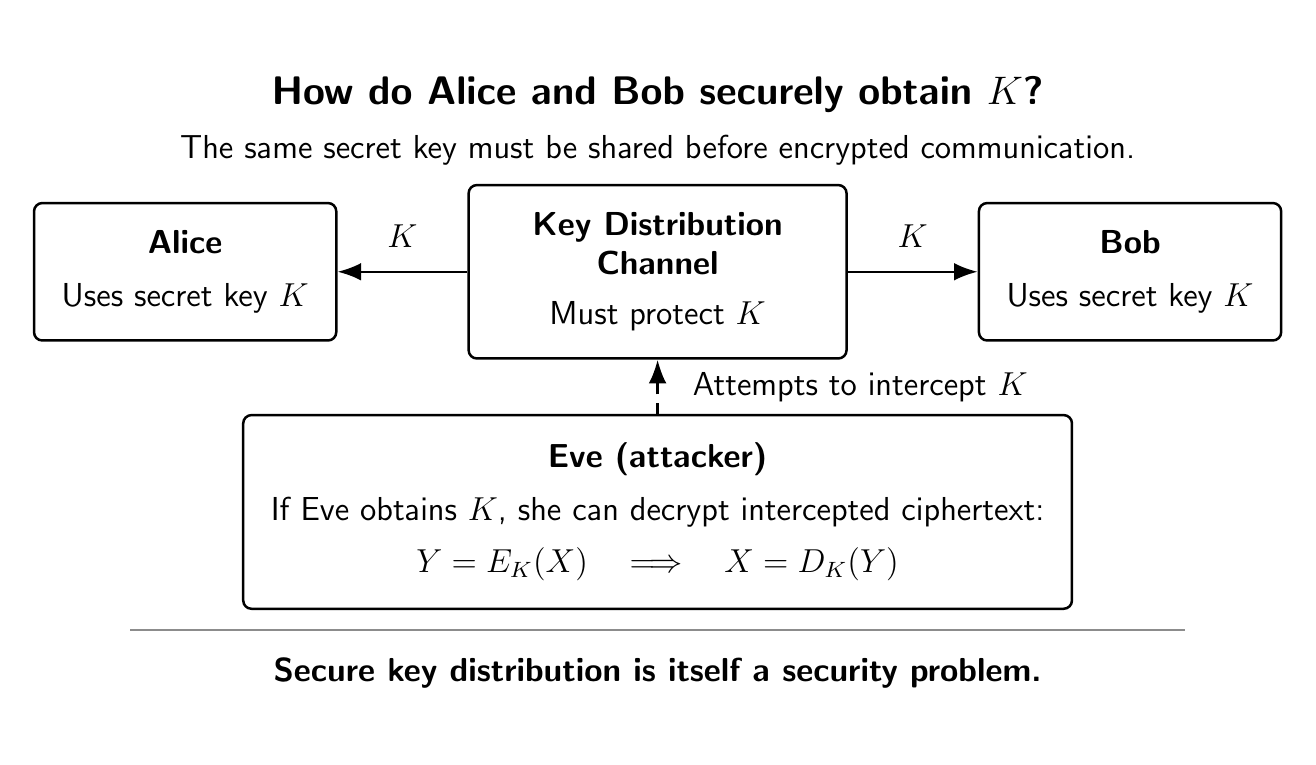
\begin{tikzpicture}[
    font=\sffamily\large,
    line width=0.9pt,
    background rectangle/.style={fill=white,draw=none},
    show background rectangle,
    box/.style={
        draw=black,fill=white,rounded corners=3pt,
        align=center,inner sep=10pt
    },
    party/.style={box,minimum width=3.4cm,minimum height=1.65cm},
    channel/.style={box,minimum width=4.8cm,minimum height=1.65cm},
    arrow/.style={-{Latex[length=3mm]},line width=0.9pt},
    threat/.style={arrow,dash pattern=on 4pt off 3pt},
    note/.style={align=center,font=\sffamily\large}
]
% A fixed, near-16:9 canvas keeps labels legible on slides and the web.
\path[use as bounding box] (-8,-4.5) rectangle (8,4.5);

\node[font=\sffamily\Large\bfseries,align=center] at (0,3.65)
    {How do Alice and Bob securely obtain $K$?};
\node[note] at (0,2.95)
    {The same secret key must be shared before encrypted communication.};

\node[party] (alice) at (-6,1.4)
    {\textbf{Alice}\\[5pt]Uses secret key $K$};
\node[channel] (channel) at (0,1.4)
    {\textbf{Key Distribution}\\\textbf{Channel}\\[4pt]Must protect $K$};
\node[party] (bob) at (6,1.4)
    {\textbf{Bob}\\[5pt]Uses secret key $K$};

% Both arrows represent obtaining the same K, not two different keys.
\draw[arrow] (channel.west) -- node[above=5pt] {$K$} (alice.east);
\draw[arrow] (channel.east) -- node[above=5pt] {$K$} (bob.west);

\node[box,minimum width=8.9cm,minimum height=1.85cm] (eve) at (0,-1.65)
    {\textbf{Eve (attacker)}\\[5pt]
     If Eve obtains $K$, she can decrypt intercepted ciphertext:\\[5pt]
     $Y=E_K(X)\quad\Longrightarrow\quad X=D_K(Y)$};

% Dashed direction indicates an attempted interception, not a legitimate
% key delivery or a guarantee that an attack succeeds.
\draw[threat] (eve.north) -- node[right=9pt,align=left]
    {Attempts to intercept $K$} (channel.south);

\draw[black!45,line width=0.6pt] (-6.7,-3.15) -- (6.7,-3.15);
\node[note,font=\sffamily\large\bfseries] at (0,-3.7)
    {Secure key distribution is itself a security problem.};
\end{tikzpicture}
\end{document}
